\label{microSD}

Zunächst sollten die gemessenen CO$_2$-Werte auf dem Arduino selbst abgespeichert werden. Der EEPROM wäre dafür die Lösung gewesen. Jedoch besitzt dieser eine Speicherkapazität von 1KB. Bei größeren Messungen reicht das unter Umständen nicht aus, sodass eine Methode gefunden werden musste, in welcher die Daten extern vom Arduino abgespeichert werden können. \\
Dazu haben wir den, in Abbildung \ref{fig:SD-Modul} zu sehenden Mikro-SD-Karten-Adapter hinzugezogen. Hier können die gemessenen CO$_2$-Werte ohne Speicherprobleme gesichert werden. \\

\begin{figure}[!hbt]
	\centering
	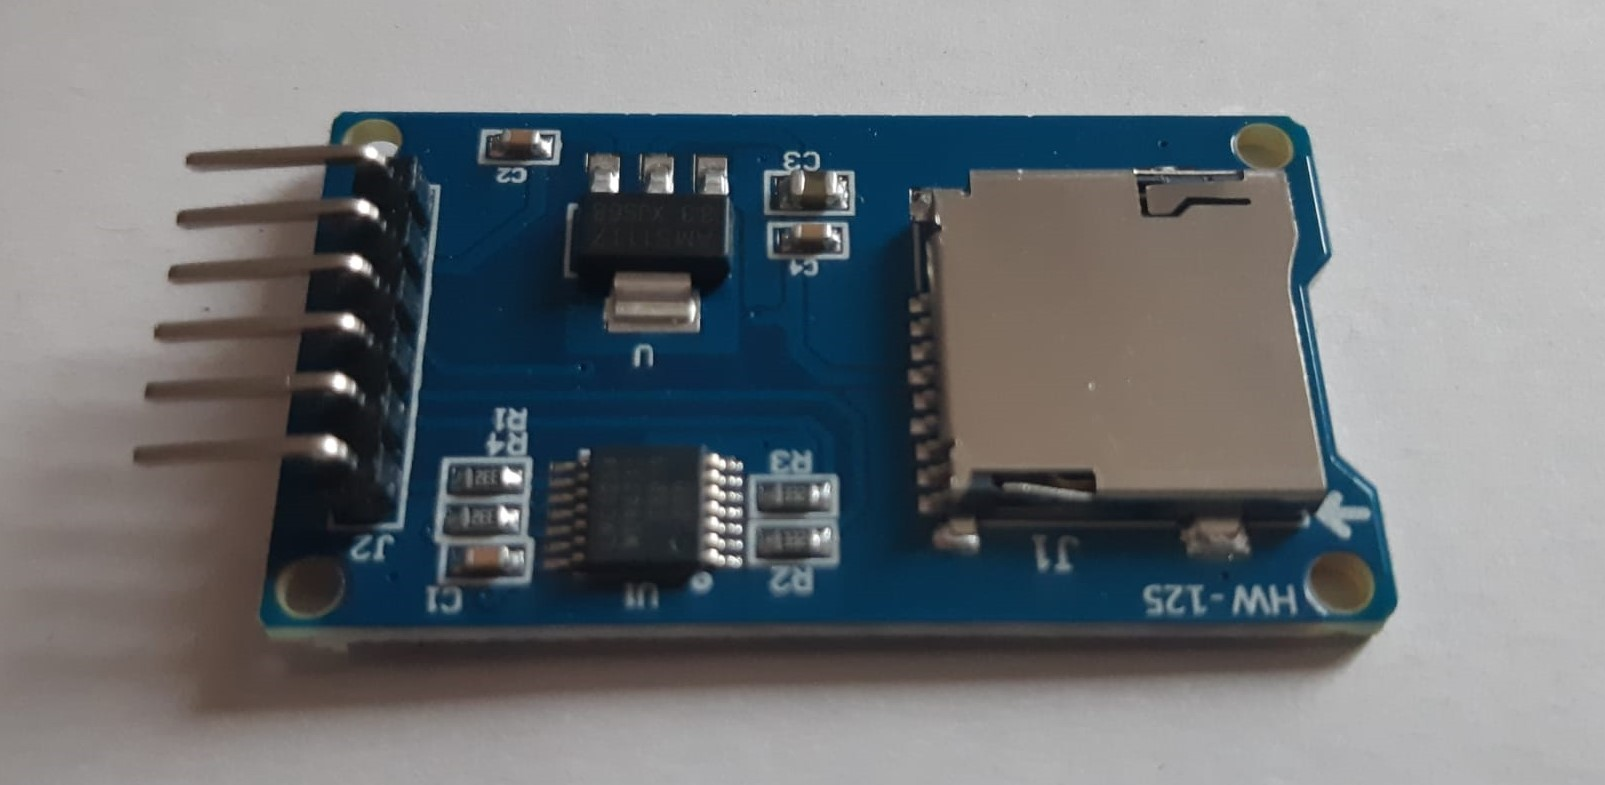
\includegraphics[width=0.7\linewidth]{Images/Mikro-SD_2}
	\footnotesize{\\ Quelle: eigene Aufnahme}
	\caption{Verwendeter Mikro-SD-Karten-Adapter, Bild von der Vorderseite aufgenommen}
	\label{fig:SD-Modul}
\end{figure}

Der Mikro-SD-Karten-Adapter ist über die, in Abbildung \ref{fig:SD-Modul_RUCK} zu sehenden PINs MISO, MOSI, SCK und CS, mit dem Arduino verbunden. Die komplementären PINs des Arduinos sind in Abbildung \ref{fig:Layout} zu sehen. Der Adapter benötigt zudem eine Versorgungsspannung von mindestens $4,5\volt$ bis maximal $5,5\volt$ zur Masse. \cite[vgl. S. 1]{ebaySearch.} \\

\begin{figure}[!hbt]
	\centering
	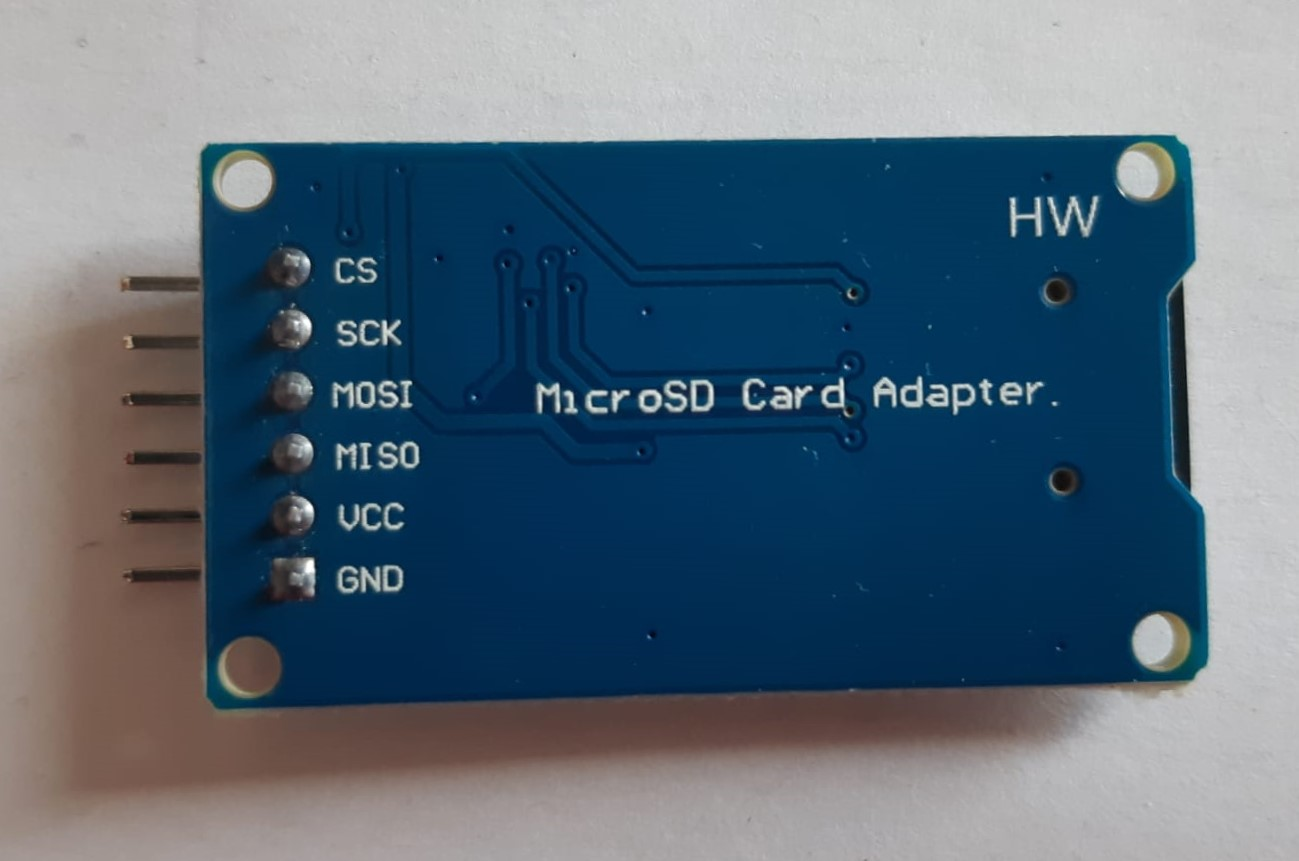
\includegraphics[width=0.6\linewidth]{Images/Mikro-SD_3}
	\footnotesize{\\ Quelle: eigene Aufnahme}
	\caption{Verwendeter Mikro-SD-Karten-Adapter, Bild von der Rückseite aufgenommen}
	\label{fig:SD-Modul_RUCK}
\end{figure}

Für die Integration der SD-Karte, muss zunächst die Bibliothek <SD.h> eingebunden werden. Anschließend wird eine globale Variable als File deklariert. In unserem Programmablauf wird die anschließende Initialisierung der SD-Karte zweimal durchgeführt. Das erste mal im Setup, vor dem Programmablauf. Die Begründung liegt darin, dass dem Benutzer bei fehlender SD-Karte schon vor der Auswahl des Messmodus eine Fehlermeldung angezeigt werden kann. 

\begin{figure}[!hbt]
	\centering
	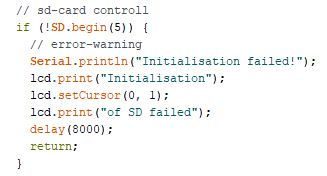
\includegraphics[width=0.6\linewidth]{Images/sdSetup}
	\footnotesize{\\ Quelle: eigene Aufnahme}
	\caption{Codeausschnitt zur Initialisierung der SD-Karte im Setup aus dem Quellcode}
	\label{fig:SD_Setup}
\end{figure}

